\subsection{Introducci\'on} 

En este ejercicio se nos pide encontrar un algoritmo que encuentre una combinacion de vuelos entre la ciudad $A$ y la ciudad $B$ tal que encuentre la manera de llegar lo antes posible a destino.

La entrada del algoritmo ser\'a:

\begin{itemize}
\item Un string \textbf{A} $\rightarrow$ Representar\'a la ciudad de partida.
\item Un string \textbf{B} $\rightarrow$ Representar\'a la ciudad de de llegada.
\item Un entero \textbf{n} $\rightarrow$ Representar\'a el numero total de vuelos entre todas las ciudades.
\item \textbf{n} filas donde, para cada fila se tiene:
\begin{itemize}
\item Un string \textbf{ori} $\rightarrow$ Representar\'a la ciudad de partida.
\item Un string \textbf{des} $\rightarrow$ Representar\'a la ciudad de de llegada.
\item Un entero \textbf{ini} $\rightarrow$ Representar\'a el numero la hora de despegue de la ciudad $ori$
\item Un entero \textbf{fin} $\rightarrow$ Representar\'a el numero la hora de arribo a la ciudad $des$
\end{itemize}
\end{itemize}

A esto nuestro algoritmo deve devolver:
\begin{itemize}
\item Un entero \textbf{fin} $\rightarrow$ Representar\'a el horario de llegada a la ciudad $B$.
\item Un entero \textbf{k} $\rightarrow$ la cantidad de vuelos del itinerario.
\item $k$ enteros \textbf{v_1, v_2 ..., v_k} $\rightarrow$ los vuelos tomados
\end{itemize}

\subsection{Ejemplos y Soluciones}
Se procede a generar una posible instancia del problema para ilustrar lo que se espera del algoritmo.

Supongamos que queremos ir de la ciudad de Buenos Aires a la isla de Saba (Dato curioso: en la isla de Saba se encuentra el aeropuerto mas chico del mundo (400 m)).

Lamentablemente no existen vuelos directos, por lo que tendrémos que hacer escala para poder llegar ahí. A continuaíón se muestran los posibles vuelos que podríamos tomar para llegar a destino.

\begin{itemize}
\item Buenos Aires - Seúl: 10 - 20
\item Buenos Aires - La isla de los pitufos: 17 - 24
\item Seúl - San Fransisco: 22 - 40
\item La isla de los pitufos - isla de Saba: 28 - 30
\item San Fransisco - isla de Saba: 40 - 43
\item Buenos Aires - San Fransisco: 13 - 20
\end{itemize}

Luego, podemos observar que existen muchas maneras factibles de llegar desde Buenos Aires al objetivo. Una manera es tomar la ruta de Buenos aires - Seul, de allí ir a San Fransisco y finalmente a la isla de Saba, pero rapidamente vemos que si bien este viaje es factible, es al menos tan bueno como tomar el vuelo de Buenos aires a san fransisco y de allí continuar a Saba. De esta observación se desprende un dato interesante que utilizaremos en nuestro algoritmo, si se llegar de la manera mas barata a un grupo de ciudades $v_1$, $v_2$, ... $v_s$ y tengo $w_1$, $w_2$,...$w_i$ ciudades a las que puedo llegar desde el primer grupo. Si ahora tomo la ciudad $w_g$ tal que la hora de arribo a esa ciudad desde una en $v$ es la menor posible, sé que no es posible llegar de una manera mas barata a esa ciudad tambien.

Rapidamente esta idea nos remite al algoritmo de dijstra, el cual comparte una gran similitud en la idea de ir explorando todos los caminos más cortos que parten del vértice origen y que llevan a todos los demás vértices hasta llegar al destino, por lo que mas adelante intentaremos valernos de esta idea.

Luego de esta gran revelación algoritmica, continuamos con el problema que nos atañe. Es facil resolver a mano esta instancia del problema y descubrir que la combinación de vuelos optima es:
\begin{itemize}
\item Buenos Aires - La isla de los pitufos: 17 - 24
\item La isla de los pitufos - isla de Saba: 28 - 30
\end{itemize}
Llegando a destino a la hora $30$.

\subsection{Desarrollo}
Como ya hemos adelantado en el apartado anterior, la idea subyacente en este problema es, utilizando un algoritmo de dijstra levemente modificado, en cada paso, calcular la manera mas barata de llegar desde un conjuto de ciudades ya visitadas, a uno quue todavía no hemos visitado.

==COMPLETAR==

\subsection{Complejidad}

Dado que el algoritmo consiste en iterar por dos loops anidados, cuyo tamaño es $n$ (osea, la cantidad de vuelos), la compelgidad del algoritmo será $O(n^2)$.

Ademas, este algoritmo para cada paso del loop mas externo, itera forzosamente por todo el arreglo para determinar el minimo, por lo que sabemos que, para el caso en que existe una solución $\omega (n^2)$.

\subsection{Experimentacion}

Dado que ya dijimos que no existen, 'peores casos', porque nuestro algoritmo esta acotado por ambos lados por $n^2$, realizamos un testeo random para comprobarlo:

\begin{figure}[h!]
  \begin{center}
	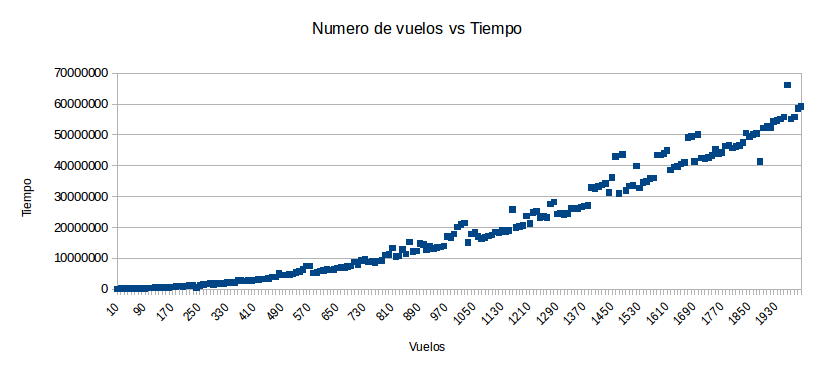
\includegraphics[scale=0.5]{Ej1/testingnvst.png}
	%\caption{Descripcion de la figura}
	\label{nombreparareferenciar}
  \end{center}
\end{figure}

Aqui puede verse claramente que nuestras hipotesis eran correctas.